\documentclass[12pt]{article}
\usepackage{amsmath, amssymb, amsthm}
\usepackage[margin=1in]{geometry}
\usepackage{graphicx, enumitem}
\usepackage{tikz, fancyhdr}
\usepackage[labelfont=bf]{caption}

\pagestyle{fancy}
\fancyhf{}
\chead{PROBLEM SET 8}
\rhead{Elliot Ahn}
\lhead{Machine Learning}
\rfoot{\thepage}

\setlength{\headheight}{15pt}
\renewcommand{\footrulewidth}{0.5pt}

\newcommand{\Ein}{E_{\text{in}}}
\newcommand{\Eout}{E_{\text{out}}}
\newcommand{\x}{\mathbf{x}}
\newcommand{\E}{\mathbb{E}}

\begin{document}

\begin{enumerate}[leftmargin=*]
\item (e) A polynomial in $x, y$ of order $r$ has $r + 1$ terms with power $r$. For example, $r = 2$ yields 3 quadratic terms: $x^2$, $xy$, and $y^2$. Therefore, a polynomial of order $r$ has (excluding the constant term)
\[ (1 + 1) + (2 + 1) + \cdots + (r - 1 + 1) + (r + 1) \qquad \text{terms}. \]
This is
\[ r + \frac{r ( r + 1)}{2} \qquad \text{terms}. \]
In the case $r = 10$, this is
\[ 10 + 5 \cdot 11 = 65 \qquad \text{terms} \]
\item (d) In Logistic regression, we take a linear signal $s = \mathbf w \cdot \mathbf x$ and place it in a sigmoid and take a sign.
\[ y = \text{sgn} \left( \frac{1}{1 + e^{-s}} \right). \]
This is clearly not linear, and so taking expectation values (which is linear) would not guarantee that our resulting signal is logistic.
\item (d) In overfitting, we tend to fit the noise instead of estimating results that are out-of-sample. This tends to give a small $\Ein$ and a large $\Eout$. The goal is to get a small $\Eout$, so we do not really care if we have a larger $\Ein$. In fact, we will always choose a hypothesis that yields a larger $\Ein$ at the expense of a smaller $\Eout$. As a result, measuring $\Eout - \Ein$ does not say if we are overfitting. Yes, it is true that as we overfit, $\Eout - \Ein$ increases. However, in the opposite spectrum, if we are underfitting, $\Eout - \Ein$ can be pretty small, however increasing the complexity of our hypothesis can increase $\Eout - \Ein$ while decreasing $\Eout$ simultaneously. Therefore, we cannot determine overfitting by only comparing $\Eout - \Ein$.
\item (d) Stochastic noise is noise due to random fluctuations and not due to the nature of the target function.
\item (a) $\mathbf w_{\text{lin}}$ minimizes the mean-squared error without any constraints. If $\mathbf w_{\text{lin}}$ minimizes the mean-squared error while also satisfying the constraint, then it must be the minimum in the constraint-region.
\item (b) Suppose we want to minimize
\[ \Ein = \frac{1}{N} (\mathbf Z \mathbf w - \mathbf y)^T (\mathbf Z \mathbf w - \mathbf y) \]
with respect to the constraint
\[ \mathbf w^T \Gamma^T \Gamma \mathbf w \leq C. \]
From KKT Lagrange multipliers, we have
\[ \nabla \Ein \propto 2 \Gamma^T \Gamma \mathbf w \]
implying that we can minimize without constraint
\[ E_{\text{aug}} = \frac{1}{N} (\mathbf Z \mathbf w - \mathbf y)^T (\mathbf Z \mathbf w - \mathbf y) + \frac{\lambda}{N} \mathbf w^T \Gamma^T \Gamma \mathbf w. \]
\item (d) 8 vs ALL had the lowest $\Ein$ with $\lambda = 1$ at 0.074.
\item (b) 1 vs ALL had the lowest $\Eout$ with $\lambda = 1$ at 0.02.
\item (e) $\Eout = 0.07972$ without the transform and $\Eout = 0.07922$ with the transform.
\item When comparing the 1 vs 5 classifier between $\lambda = 0.01$ and $\lambda = 1$, we see that the $\lambda = 0.01$ has a lower $\Ein$ but a higher $\Eout$, implying that we have overfitting.
\item 
\begin{figure}[t]
\centering
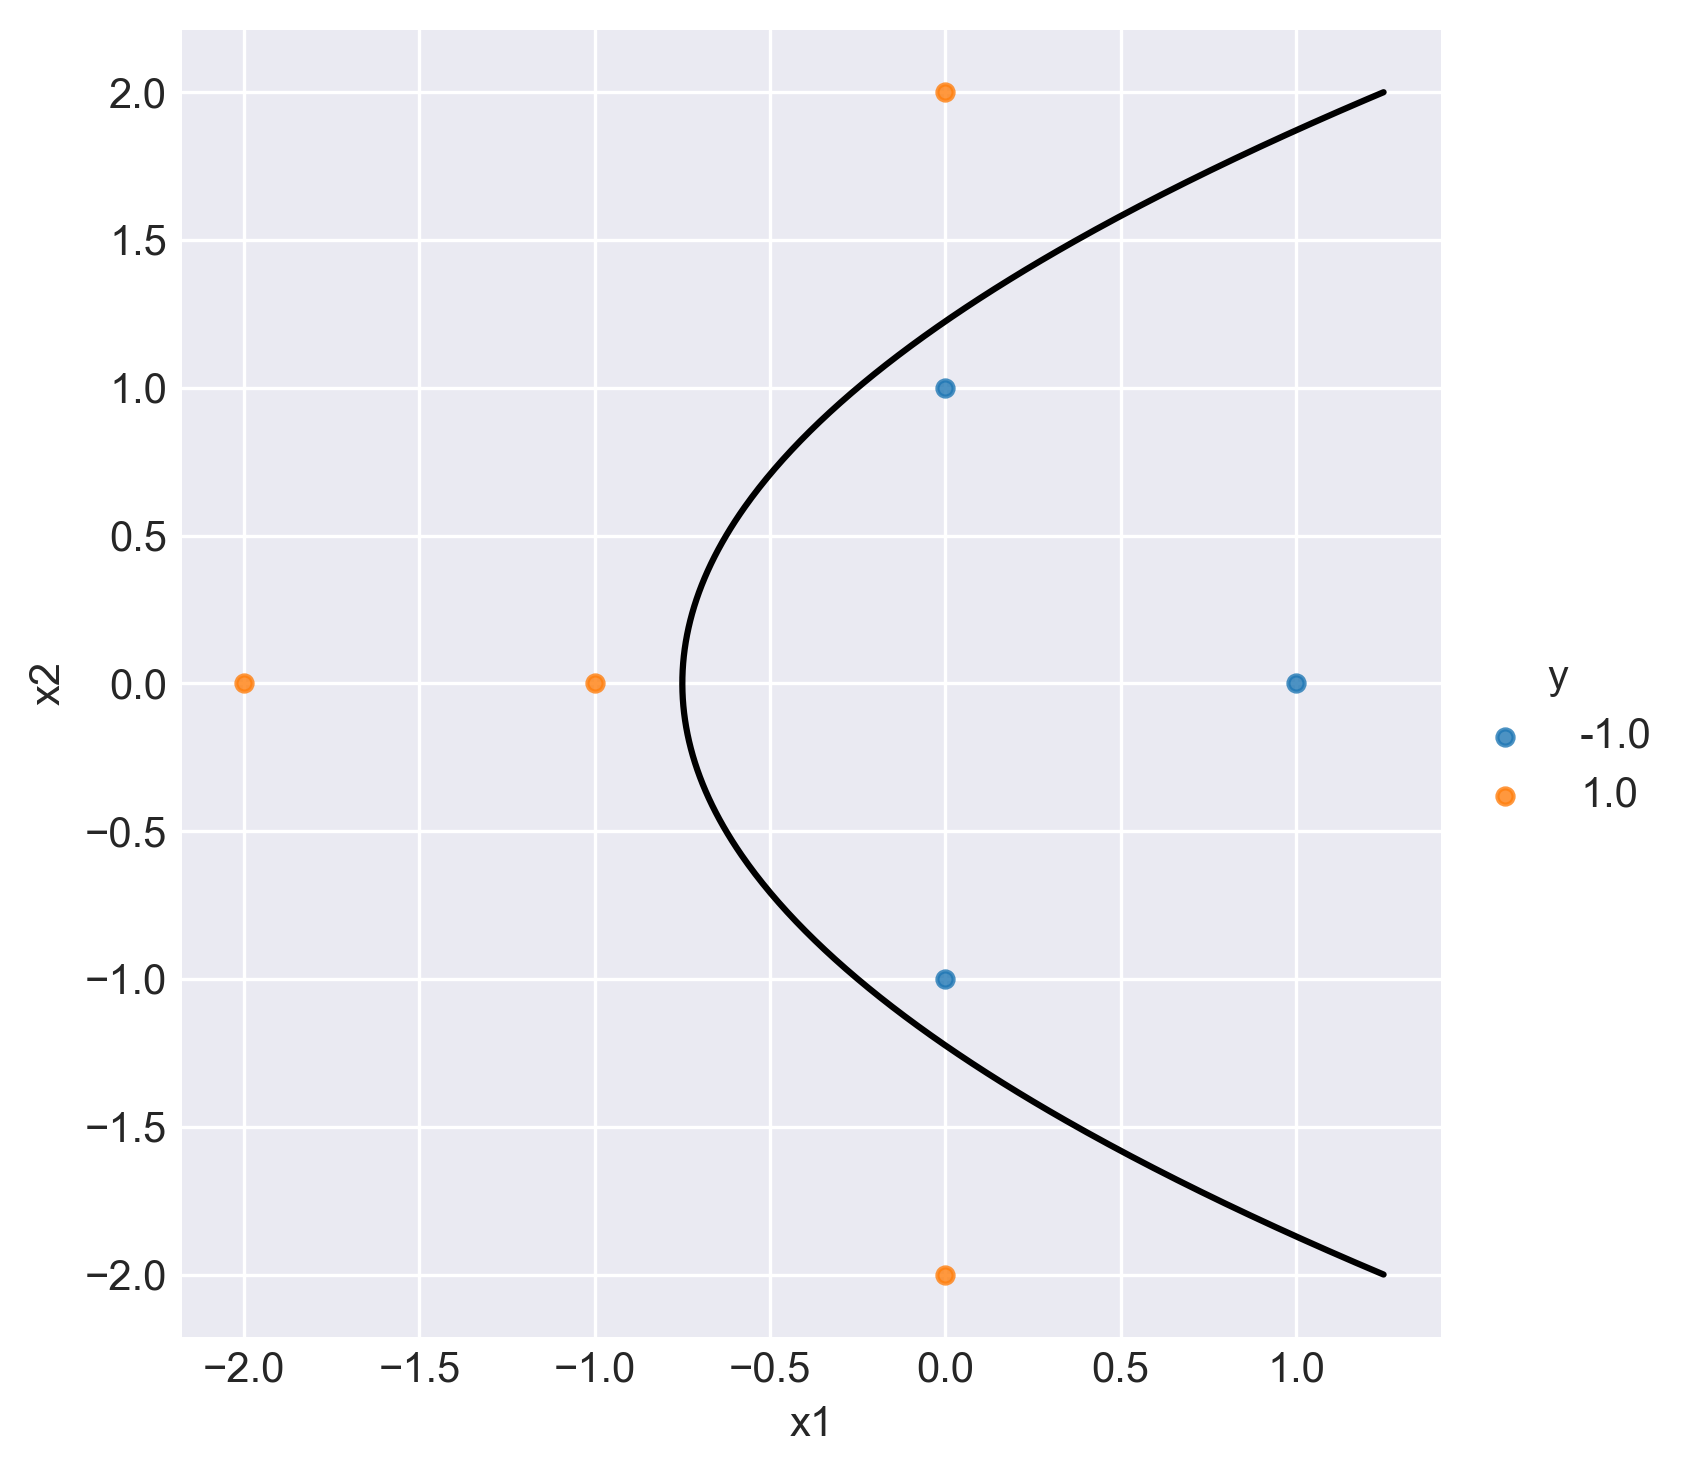
\includegraphics[scale=0.9]{support_vec_plot.png}
\caption{Problem 11} \label{Problem 11}
\end{figure} (c) We see from Figure \ref{Problem 11} that our desired solution should look something like a parabola given that the transformation is quadratic. Given the symmetry of our datapoints, we should expect our separating curve to be symmetric about the $x_2 = 0$ axis. Solving $\mathbf w^T \mathbf z + b = 0$, we get
\[ w_1 (x_2^2 - 2 x_1 - 1) + w_2 (x_1^2 - 2 x_2 + 1) + b = 0 \]
By imposing our symmetry condition, the vertex of our parabola must be along the $x_2 = 0$  axis, so we force the linear term of $x_2$ to be zero so that $w_2 = 0$. Therefore,
\[ 2 x_1 = x_2^2 + \frac{b}{w_1} - 1 \]
We want to obtain the ratio $b / w_1$. The minimum value of this ratio would be when the vertex of the parabola touches $(x_1, x_2) = (-1, 0)$. This yields
\[ \left( \frac{b}{w_1} \right)_{\text{min}} = - 1 \]
The maximum value of this ratio would be when the parabola hits $(0, \pm 1)$. This gives
\[ \left( \frac{b}{w_1} \right)_{\text{max}} = 0 \]
The separating curve given by SVMs that maximizes the margin would be the midpoint of these two ratios, so that
\[ \left( \frac{b}{w_1} \right)_{\text{SVM}} = -0.5 \]
so $w_1 = 1$ and $b = -0.5$.
\item The Lagrangian we would like to maximize is given by
\[ \mathcal L (\mathbf \alpha) = \sum_{n = 1}^N \alpha_n - \frac{1}{2} \sum_{n = 1}^N \sum_{m = 1}^N y_n y_m \alpha_n \alpha_m K_{n m} (\mathbf x_n^T \mathbf x_m) \]
where $K_{nm}(\mathbf x_n, \mathbf x_m) = (1 + \mathbf x_n^T \mathbf x_m)^2$ subject to the constraints
\[ \alpha_n \geq 0 \qquad \text{and} \qquad \sum_{n = 1}^N \alpha_n y_n = 0.\]
When running SVM on this data, we have 5 support vectors with values
\[ \alpha_1 = 0, \alpha_2 = 0.4857, \alpha_3 = 0.92, \alpha_4 = 0.8887, \alpha_5 = 0.15, \alpha_6 = 0.36, \alpha_7 = 0. \]
\item (a) When training on only 100 samples, $\Ein = 0$ with probably almost $1.$
\item (e) The kernel form beats the regular form 91 percent of the time.
\item (d) The kernel form beats the regular form 83 percent of the time.
\item (d) On average, $\Ein$ and $\Eout$ both go down.
\item (c) On average, $\Ein$ and $\Eout$ both go up.
\item (a) $\Ein$ is almost never 0.
\item (b) The value of $f$ is our parameter we would like to estimate. It follows some probability distribution $g(f) \, df$, and we have from Bayes' rule
\[ g(f \, | \, x = 1) \, df = \frac{g(f) p(x = 1 \, | \, f) \, df}{p(x = 1)} = \frac{g(f) p(x = 1 \, | \, f) \, df}{\int_0^1 df \, p(x = 1 \, | \, f) g(f)} \]
Now $g(f) = 1$ since we assumed it's a continuous prior, and $p(x = 1 \, | \, f) = f$. Therefore,
\[ g(f \, | \, x = 1) \, df = 2 f \, df \]
so that
\[ g(f \, | \, x = 1) = 2 f \]
\item (c) The MSE of $g_1(\x), g_2(\x)$ are
\[ \text{MSE}(g_i(\x)) = \E [(g_i - f)^2] = \E [ g_i^2] + f^2 - 2 \hat g_i f \]
So the average of these MSE's is
\[ \frac{1}{2} \E[g_1^2 + g_2^2] + f^2 - (\hat g_1 + \hat g_2) f\]
If we take the MSE of $(g_1 + g_2) / 2$, then
\begin{align*}
\text{MSE} \left[ \frac{1}{2} \left( g_1 + g_2 \right) \right] &= \E \left[ \left( \frac{1}{2} \left( g_1 + g_2 \right) - f \right)^2 \right] \\
&= \E \left[ \frac{1}{4} g_1^2 + \frac{1}{4} g_2^2 + \frac{1}{2} g_1 g_2 - (g_1 + g_2) f + f^2 \right]
\end{align*}
If we subtract this from the average of the MSEs, then we get
\[ \frac{1}{2} \left(\text{MSE}(g_1) + \text{MSE}(g_2) \right) - \text{MSE} \left[ \frac{1}{2} \left( g_1 + g_2 \right) \right] = \frac{1}{2} \E \left[ g_1^2 + g_2^2 - g_1 g_2 \right] \geq 0 \]
since $x^2 + y^2 - x y \geq 0$ for all $x, y$.
\end{enumerate}

\end{document}